\documentclass{article}

\usepackage[normalem]{ulem}
\usepackage{fancyhdr}
\usepackage[parfill]{parskip}
\usepackage{tikz}
\pagestyle{fancyplain}

\title{Oscillations}
\author{Todd Davies}
\date{\today}

\begin{document}

\rhead{Oscillations}
\lhead{\today}

\maketitle

\section*{What's an oscillation?}
\thispagestyle{empty}
An oscillation is defined as a '\textit{A repetitive back and forth motion}' (an object that oscillates can also be said to vibrate).

\section*{Equations you need to know}
\begin{itemize}
	\item The angular velocity is related to the time period of the oscillation with the following equation:
	\[
		\omega = \frac{2 \pi}{T}
	\]
	Which is of course equal to:
	\[
	 \omega = 2 \pi f
	\]
	\item In simple harmonic motion, displacement can be calculated using the following:
	\[
		x = A \sin (2 \pi ft)
	\]
	or
	\[
		x = A \cos(2 \pi ft)
	\]
	\item The acceleration of a body undergoing simple harmonic motion is proportional to it's displacement from the equlibrium position:
	\[
		a \propto x
	\]
	We can include the constant in the equation to give:
	\[
		a = -(2 \pi f)^{2}x
	\]
	\item The maximum speed of an object undergoing simple harmonic motion can be found using:
	\[
		v_{max} = (2 \pi f)A
	\]
\end{itemize}

The quantities and their respective units are shown in this table:

\begin{center}
	\begin{tabular}{|l|l|l|}
		\hline
			Quantity & Abbreviation & Unit \\ \hline
			Time period & $T$ & Second ($s$) \\ \hline
			Frequency & $f$ & Hertz ($Hz$) \\ \hline
			Acceleration & $a$ & Metres per second squared ($ms^{-2}$) \\ \hline
			Time & $t$ & Seconds($s$) \\ \hline
			Angular velocity & $\omega$ & Radians per second($rad/s$) \\ \hline
			Amplitude & $A$ & Meters ($m$) \\ \hline
			Velocity & $v$ & Meters per second ($ms^{-1}$) \\ \hline
			Displacement & $x$ & Meters ($m$) \\ \hline
	\end{tabular}
\end{center}

\section*{Types of oscillation}
There are two types of oscillation - free and forced.
\subsection*{Free oscillations}
This is when an object is left to vibrate at it's \textit{natural frequency}. The oscillating object is under no external influence (other than the influence that initiated the motion). 

An example of a free oscillation could be when you pluck a violin string. The string oscillates at its natural frequency which produces the note that you hear.
\subsection*{Forced oscillations}
A forced oscillation is when an object moves back and forth under the influence of another driving object.

An example of this is if you wave your hand at somebody. Your arm is driving your hand, but your hand isn't moving at it's natural frequency.

\section*{Describing an oscillation}
Oscillations have maximum velocity at the point where their displacement is zero. At this point, they have minimum acceleration.
Oscillations have maximum acceleration at the point where their displacement is maximum. At this point they have minimum velocity.
The shape of a graph plotting displacement against time is going to be something like:

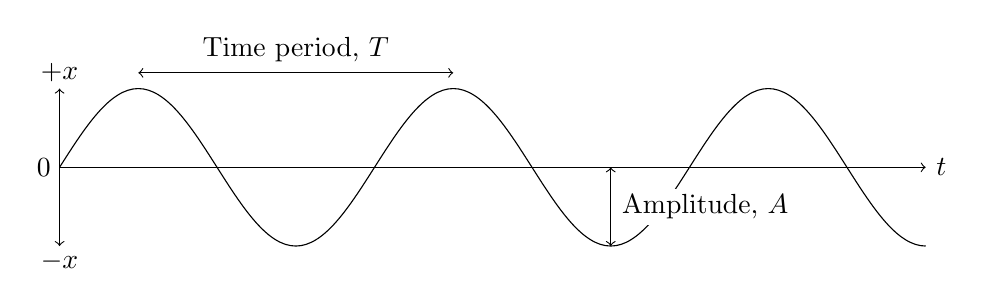
\begin{tikzpicture}
	%curve
		\draw (0.5,0) sin (1.5,1) cos (2.5,0) sin (3.5,-1) cos (4.5,0) sin (5.5,1) cos (6.5,0) sin (7.5,-1) cos (8.5,0) sin (9.5,1) cos (10.5,0) sin (11.5,-1);
	% zero crossing
		\draw[dotted] (0.5,0) -- (11.5,0);
	%axis + labels
		\draw [<->] (0.5,1) -- (0.5,-1);
		\draw [->] (0.5,0) -- (11.5,0);
		\node at (11.7,0) {$t$};
		\node at (0.5,1.2) {$+x$};
		\node at (0.5,-1.2) {$-x$};
		\node at (0.3,0) {$0$};
	%Time period description
		\draw [<->] (1.5,1.2) -- (5.5,1.2);
		\node at (3.5,1.5) {Time period, $T$};
	%Amplitude description
		\draw [<->] (7.5,0) -- (7.5,-1);
		\draw [fill=white,ultra thick,white] (7.6,-0.3) rectangle (9.7,-0.7); %to stop line overlap
		\node at (8.7, -0.5) {Amplitude, $A$};
\end{tikzpicture}

This graph can be described as \textit{sinusoidal}.

\section*{Phase}
As you should know from the G482 module, waves have a phase. The phase of a wave is the point an oscillating mass has reached in it's cycle of oscillation. Phase is measured in degrees or radians. Two waves can have a phase difference, also measured in degrees or radians.

Here is a diagram of two identical waves out of phase by 180 degrees:

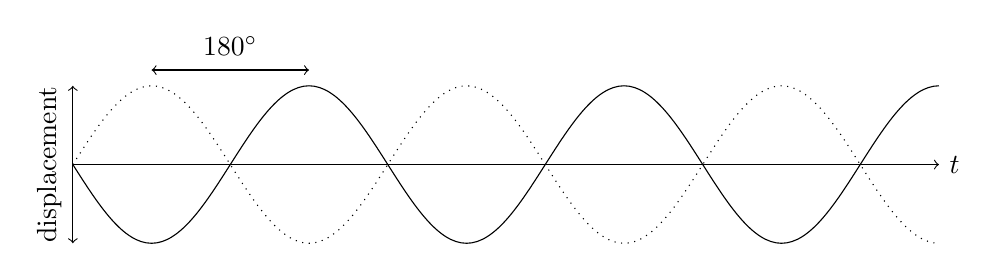
\begin{tikzpicture}
	%curve 1
		\draw[dotted] (0.5,0) sin (1.5,1) cos (2.5,0) sin (3.5,-1) cos (4.5,0) sin (5.5,1) cos (6.5,0) sin (7.5,-1) cos (8.5,0) sin (9.5,1) cos (10.5,0) sin (11.5,-1);
	%curve 2
		\draw (0.5,0) sin (1.5,-1) cos (2.5,0) sin (3.5,1) cos (4.5,0) sin (5.5,-1) cos (6.5,0) sin (7.5,1) cos (8.5,0) sin (9.5,-1) cos (10.5,0) sin (11.5,1);
	% zero crossing
		\draw[dotted] (0.5,0) -- (11.5,0);
	%axis + labels
		\draw [<->] (0.5,1) -- (0.5,-1);
		\draw [->] (0.5,0) -- (11.5,0);
		\node at (11.7,0) {$t$};
		\node[rotate=90] at (0.2,0) {displacement};
	%Phase difference description
		\draw [<->] (1.5,1.2) -- (3.5,1.2);
		\node at (2.5,1.5) {$180^\circ$};
\end{tikzpicture}

\textit{N.b. 180 degrees is equal to $\pi$ radians.}

\end{document}